\documentclass{weekly}
\begin{document}
\maketitlew{Аналитическая механика}{1}{2}{5}

\paragraph{3.6.} Плоская фигура движется в~своей плоскости.
Найти положение точки~$A$, если известны скорость этой точки~$\vec v_A$,
скорость некоторой другой точки~$\vec v_0$ и~угловая скорость
фигуры~$\vec\omega$. Использовать полученный результат для~определения
положения мгновенного центра скоростей~$P$.

$\blacktriangleright$ По~теореме о~распределении скоростей
в~твёрдом теле
\begin{equation}\label{3.6:vA}
    \vec v_A = \vec v_0 + \vec\omega \times \overline{OA}.
\end{equation}
Умножим векторно уравнение~\eqref{3.6:vA} на~$\vec\omega$ слева:
\begin{gather}
    \vec\omega \times \left(\vec v_A - \vec v_0\right) =
            \vec\omega \times \vec\omega \times \overline{OA}
        = \vec\omega \cancelto{0}
            {\left(\vec\omega, \overline{OA}\right)}\quad -
            \overline{OA} \left(\vec\omega, \vec\omega\right)
        = -\omega^2 \cdot \overline{OA}; \\[\parskip]
    \overline{OA} = \frac{\vec\omega \times
            \left(\vec v_0 - \vec v_A\right)}{\omega^2}.
\end{gather}
В~частности, для~мгновенного центра скоростей~$P$ можно записать
$\vec v_P = \vec 0$.\\[-\parskip]

\textbf{Ответ:}\quad $\overline{OA} = \dfrac{\vec\omega \times
\left(\vec v_0 - \vec v_A\right)}{\omega^2}$;\qquad
$\overline{OP} = \dfrac{\vec\omega \times \vec v_0}{\omega^2}$.
\hfill $\blacktriangleleft$


\begin{wrapfigure}[8]{r}{4.5cm}\vspace{-6mm}
    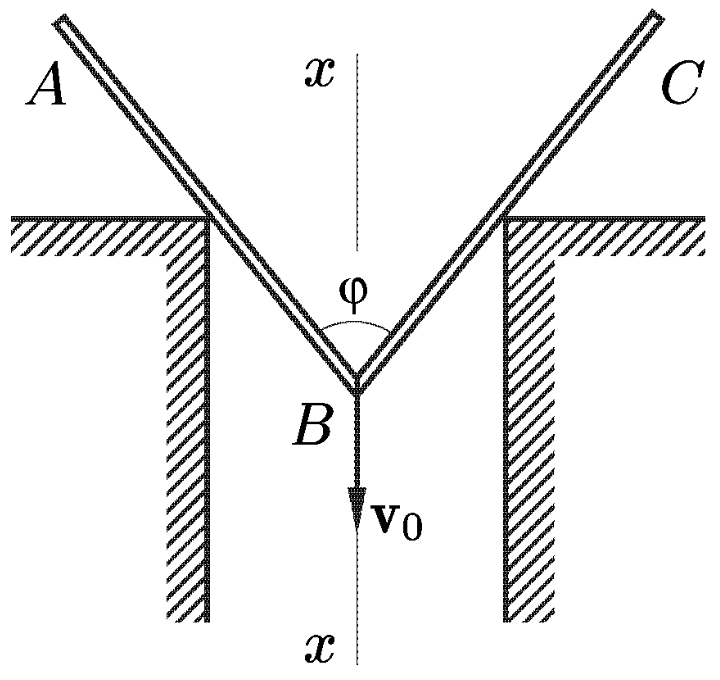
\includegraphics[width=4.5cm]{3-12}
\end{wrapfigure}
\paragraph{3.12.} Стержни~$AB$ и~$BC$ шарнирно соединены в~точке~$B$
и~опираются на~два прямых угла, как~показано на~рисунке.
Точка~$B$ движется по~прямой~$xx$, равноудалённой от~вертикальных сторон
углов. Во~время движения стержни касаются вершин прямых углов.
Доказать, что~скорость точки касания каждого стержня вершин прямого угла
направлена вдоль стержня. Найти также скорости этой точки в~зависимости
от~угла~$\angle ABC = \varphi$, если~скорость точки~$B$ равна~$v_0$.

$\blacktriangleright$ Введём неподвижную систему координат~$T\xi\eta$
в~точке~$T$ касания стержнем угла в~данный момент времени;
ось~$\xi$ направим вдоль стержня,
ось~$\eta$~--- перпендикулярно названному направлению.
Точка~$T$ имеет скорость
\begin{equation}\label{3.12:vT}
    \vec v_O = v_\xi \mathbf{e_\xi} + v_\eta \mathbf{e_\eta}.
\end{equation}
Требуется показать, что~$v_\eta = 0$. В~самом деле, рассмотрим
точку~$A$ стержня с~координатами~$(\delta \xi; 0)$,
которая станет точкой касания через промежуток времени~$\delta t$.
С~одной стороны, понятно, что
\begin{equation}\label{3.12:vA}
    \vec v_A = \frac{\delta \xi}{\delta t} \,\mathbf{e_\xi};
\end{equation}
с~другой стороны, по~теореме Эйлера
\begin{equation}\label{3.12:Euler}
    \vec v_A = \vec v_T + \vec\omega \times \overline{TA}.
\end{equation}

Используя~\eqref{3.12:vT} и~\eqref{3.12:vA}, запишем~\eqref{3.12:Euler}
в~<<проекциях>>:
\begin{equation}
    \frac{\delta\xi}{\delta t} \,\mathbf{e_\xi}
        = v_\xi \mathbf{e_\xi} + v_\eta \mathbf{e_\eta} -
            \omega\,\delta\xi \cdot
            \left(\mathbf{[e_\xi \times e_\eta] \times
                \mathbf{e_\xi}}\right)
        = v_\xi \mathbf{e_\xi} + v_\eta \mathbf{e_\eta} +
            \omega\,\delta\xi \,\mathbf{e_\eta}.
\end{equation}
Таким образом, $v_\eta = \omega \,\delta\xi \to 0$,
что~и требовалось доказать. \hfill $\blacksquare$

Проекции скоростей точек стержня
на~ось~$\xi$ равны между собой (это, между прочим, побочный результат
приведённого выше доказательства). В~силу симметрии системы
нетрудно записать искомый результат.

\textbf{Ответ:}\quad $v_T = v_B \cos\dfrac{\varphi}{2}$.
\hfill $\blacktriangleleft$

\end{document}
